Acoustical measurements were taken in a $3.6 \times 2.35 \times 2.55$~m (length $\times$ width $\times$ height) anechoic chamber with 8-inch deep (equal to $1/4$ wavelength at $\sim425$~Hz) anechoic foam wedges.
We consider three source positions: $\vec{s}_\textrm{A} = (0.35,0,0)$~m, $\vec{s}_\textrm{B} = (0.35,0.35,0)$~m, and $\vec{s}_\textrm{C} = (0.35,0.7,0)$~m.
For each source,\footnote{Here, we use Genelec 8010A loudspeakers.} we measure, up to order $L_\textrm{in} = 4$, ambisonics impulse responses for all microphone positions $\vec{u} = (0, u_y, 0)$ with $u_y = [-0.5,0.5]$~m in increments of $0.05$~m.
(The impulse response measurement procedure is described in \apxref{chap:A5_Impulse_Response}.)
These microphone and source positions are illustrated in \figref{fig:10_Experimental_Validation:Experimental_Setup}.
The ambisonics impulse responses are then equalized by the frequency response of the same source measured by an omnidirectional reference microphone at the same position, thereby compensating for the directivity of the source.

% Diagram of source/mic positions
\begin{figure}[t]
\centering
  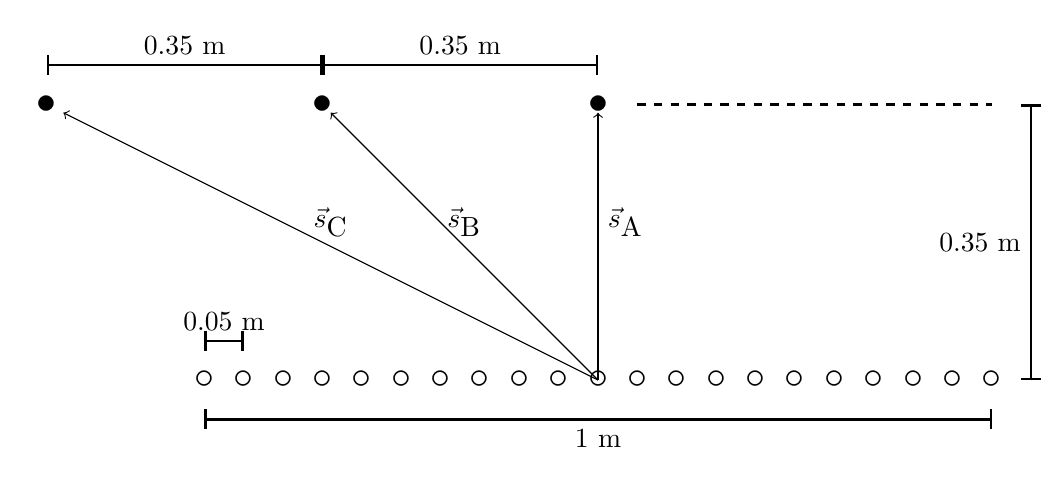
\begin{tikzpicture}[scale=10]
% Parameters
\def\radius{0.1};
\def\arrowScale{0.97};
\def\offset{0.05};

\def\micSpacing{1};
\def\micIncrement{0.05};
\def\micL{-0.5*\micSpacing};
\def\micR{0.5*\micSpacing};

\def\sourceAX{0};
\def\sourceBX{-0.35};
\def\sourceCX{-0.7};
\def\sourceY{0.35};

\pgfmathsetmacro\sourceAAzimuth{-atan(\sourceAX/\sourceY)}
\pgfmathsetmacro\sourceBAzimuth{-atan(\sourceBX/\sourceY)}
\pgfmathsetmacro\sourceCAzimuth{-atan(\sourceCX/\sourceY)}

\def\arcRadius{0.25};
\pgfmathsetmacro\arcAY{cos(-\sourceAAzimuth/2)*\arcRadius}
\pgfmathsetmacro\arcAX{sin(-\sourceAAzimuth/2)*\arcRadius}
\pgfmathsetmacro\arcBY{cos(-\sourceBAzimuth/2)*\arcRadius}
\pgfmathsetmacro\arcBX{sin(-\sourceBAzimuth/2)*\arcRadius}
\pgfmathsetmacro\arcCY{cos(-\sourceCAzimuth/2)*\arcRadius}
\pgfmathsetmacro\arcCX{sin(-\sourceCAzimuth/2)*\arcRadius}

% Coordinate system
%\draw[ultra thick,->] (0,0) -- (0,\radius);
%\draw[ultra thick,->] (0,0) -- (-\radius,0);

% Arrows
\node at (\sourceAX,\sourceY){\Large $\bullet$}; % source A
\node at (\sourceBX,\sourceY){\Large $\bullet$}; % source B
\node at (\sourceCX,\sourceY){\Large $\bullet$}; % source C
\draw[->] (0,0) -- (\arrowScale*\sourceAX,\arrowScale*\sourceY) node[above right, pos=0.5]{$\vec{s}_\textrm{A}$}; % source A
\draw[->] (0,0) -- (\arrowScale*\sourceBX,\arrowScale*\sourceY) node[above, pos=0.5]{$\vec{s}_\textrm{B}$}; % source B
\draw[->] (0,0) -- (\arrowScale*\sourceCX,\arrowScale*\sourceY) node[above, pos=0.5]{$\vec{s}_\textrm{C}$}; % source C

% Arcs
%\draw[domain=90:(90+\sourceBAzimuth)] plot ({\arcRadius*cos(\x)}, {\arcRadius*sin(\x)});
%\node at (1.15*\arcBX,1.15*\arcBY){$\varphi_\textrm{B}$};

% Mic positions
\foreach \i in {0,...,20}
{
\node at (\micL + \i*\micIncrement,0){\Large $\circ$};
}
%\node at (0,0){\Large $\circ$};
%\node at (\micL,0){\Large $\circ$};
%\node at (\micR,0){\Large $\circ$};

% Length measurements
\draw[thick,|-|] (\micL,-\offset) -- (\micR,-\offset) node[below, pos=0.5]{$1$~m};
\draw[thick,|-|] (\micL,\offset) -- (\micL+\micIncrement,\offset) node[above, pos=0.5]{$0.05$~m};
\draw[thick,|-|] (\micR+\offset,0) -- (\micR+\offset,\sourceY) node[left, pos=0.5]{$0.35$~m};
\draw[thick,dashed,-] (\micIncrement,\sourceY) -- (\micR,\sourceY);
\draw[thick,|-|] (\sourceCX,\sourceY+\offset) -- (\sourceBX,\sourceY+\offset) node[above, pos=0.5]{$0.35$~m};
\draw[thick,|-|] (\sourceBX,\sourceY+\offset) -- (\sourceAX,\sourceY+\offset) node[above, pos=0.5]{$0.35$~m};

\end{tikzpicture}
  \caption[Diagram of the experimental setup used for validation.]{
  Diagram of microphone positions (empty circles) and source positions (filled circles).}
  \label{fig:10_Experimental_Validation:Experimental_Setup}
\end{figure}

For each microphone spacing $\Delta \in [0.1,1]$~m (taken in increments of $0.1$~m) and each source position,
we estimate, using both the weighted average and proposed navigational methods (described in \secreftwo{sec:03_Navigation_Techniques:XF_Technique}{sec:08_Proposed_Method:Proposed_Techniques}, respectively), the ambisonics impulse response at each intermediate microphone position.
In all cases and at each intermediate position, we compute the following ``measured'' values: level, $\lambda'$; ABSE, $\eta'(f_c)$; localization vector,  $\vec{\nu}'$; and diffuseness, $\Psi'(f)$.
To better match the measurements, which were taken using the Eigenmike, we modify the near-field compensation filters given by \eqnref{eq:02_Acoustical_Theory:NearField_HPF} to use the following corner frequencies: $f_2 = 400$~Hz, $f_3 = 1$~kHz, and $f_4 = 1.8$~kHz (no filters are applied for orders $l = 0,1$), as specified in the EigenUnits user manual \citep[section 4.3]{EigenUnitsManual2018}.